\section{Resource controls and query-stratum selectivity}
\label{sec:structure}
\subsection{Budget matching and fixed-count index footprints}
All selectors use the same nearest-landmark partition and boundary-index code. Native landmarks are retained, and further landmarks follow a common augmentation order. Three caps are defined from the largest native index payload, with configurations chosen using bytes alone before query evaluation. Table~\ref{tab:budgets} audits the resulting 27 configurations per graph: four deterministic selectors and five random seeds at each of three caps. Graph adjacency is shared and excluded from these index-payload caps.

\begin{table}[H]
\centering\smalltablefont\setlength{\tabcolsep}{4pt}
\caption{Index caps and actual utilization across all matched-budget configurations. MiB means $2^{20}$ bytes. The query counts belong to the original candidate-selectivity cohort.}
\label{tab:budgets}
\begin{tabular}{@{}lrcrr@{}}
\toprule
Graph & Vertices & Caps (MiB), low/medium/high & Use (\%) & Queries \\
\midrule
Stanford & 255,265 & 7.78/8.95/10.11 & 95.39--100.00 & 6800 \\
Google & 855,802 & 27.82/31.99/36.17 & 95.90--100.00 & 6800 \\
in-2004 & 1,353,703 & 42.25/48.59/54.93 & 95.48--100.00 & 6800 \\
eu-2005 & 862,664 & 56.56/65.04/73.52 & 95.23--100.00 & 6800 \\
\bottomrule
\end{tabular}

\end{table}

The separate fixed-count control makes the number and mean size of pieces identical across selectors. Table~\ref{tab:structure} supplements the manuscript's candidate comparison with index and partition statistics. Random-P reports the mean of five independently constructed indexes; its candidate SD is the sample standard deviation of the five per-seed candidate means.

\begin{table}[H]
\centering\smalltablefont\setlength{\tabcolsep}{6pt}
\caption{Fixed-count index and partition statistics. Piece P99 and largest-piece size count vertices. For Random-P, each displayed statistic, including the maximum, is averaged over the five seed-specific values. Candidates are averaged over the 6,800 queries.}
\label{tab:structure}
\begin{tabular}{@{}lrrrrr@{}}
\toprule
Method & Index MiB & Piece P99 & Largest piece & Cand. ($10^3$) & Seed SD \\
\midrule
\multicolumn{6}{@{}l}{\textit{Stanford: 28,534 pieces; mean piece size 8.95}} \\
Ratio & 7.78 & 65.7 & 18,962 & 11.18 & -- \\
Ratio+ & 9.67 & 62.7 & 16,384 & 13.13 & -- \\
Degree & 10.26 & 65.0 & 13,990 & 11.84 & -- \\
CC$^2$FS & 9.95 & 60.0 & 14,902 & 13.66 & -- \\
Random-P & 9.96 & 65.3 & 12,568 & 12.12 & 0.36 \\
\midrule
\multicolumn{6}{@{}l}{\textit{Google: 212,524 pieces; mean piece size 4.03}} \\
Ratio & 27.82 & 31.0 & 1,584 & 1.73 & -- \\
Ratio+ & 29.19 & 27.0 & 3,344 & 2.19 & -- \\
Degree & 31.57 & 22.0 & 969 & 2.18 & -- \\
CC$^2$FS & 31.51 & 21.0 & 1,328 & 2.34 & -- \\
Random-P & 31.04 & 23.0 & 1,129 & 2.42 & 0.04 \\
\midrule
\multicolumn{6}{@{}l}{\textit{in-2004: 194,605 pieces; mean piece size 6.96}} \\
Ratio & 42.25 & 70.0 & 9,752 & 4.13 & -- \\
Ratio+ & 53.41 & 63.0 & 17,433 & 4.84 & -- \\
Degree & 62.99 & 59.0 & 11,481 & 4.18 & -- \\
CC$^2$FS & 62.90 & 57.0 & 12,580 & 4.29 & -- \\
Random-P & 60.17 & 60.8 & 11,165 & 4.21 & 0.09 \\
\midrule
\multicolumn{6}{@{}l}{\textit{eu-2005: 86,563 pieces; mean piece size 9.97}} \\
Ratio & 56.56 & 114.0 & 23,984 & 28.95 & -- \\
Ratio+ & 66.61 & 77.0 & 60,249 & 44.21 & -- \\
Degree & 75.53 & 75.0 & 13,975 & 34.90 & -- \\
CC$^2$FS & 75.27 & 63.4 & 25,138 & 37.84 & -- \\
Random-P & 74.53 & 71.8 & 16,896 & 35.17 & 0.66 \\
\bottomrule
\end{tabular}

\end{table}

\clearpage
\subsection{Interpreting the resource advantage}
At the common landmark count, Ratio uses less index space than each competing selector in Table~\ref{tab:structure} on all four graphs. It also returns fewer mean candidates than each competing selector, with Random-P interpreted as the five-seed mean. The candidate advantage is present at the same piece count and a smaller index footprint.

A query touches the union of pieces containing its answers, so candidate counts reflect both landmark placement and the resulting partition. Ratio's largest piece can exceed Degree's while its mean candidate count remains lower. The P99 and maximum piece sizes complement the query-level candidate measurements.

\subsection{All query strata at the lowest matched budget}
The original workload contains two start distributions: uniform starts (U) and degree-stratified starts (S). For each distribution, $h=1$ uses $|Q|=1,5,20$ with 1,000 queries per stratum; $h=2$ uses $|Q|=1,5$ with 200 queries per stratum. All selectors receive the same held-out queries and return candidates with complete recall.

\begin{figure}[H]
\centering
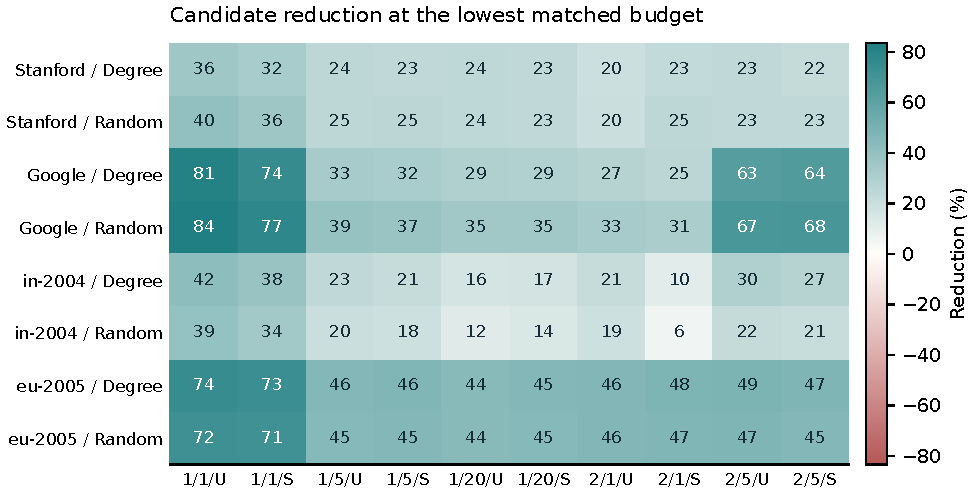
\includegraphics[width=\linewidth]{candidate_strata.pdf}
\caption{Candidate reduction, $100(1-C_{\mathrm{Ratio}}/C_{\mathrm{reference}})$, in every query stratum at the lowest matched index budget. Column labels are $h/|Q|/$start distribution. Random denotes the five-seed mean; positive values favor Ratio. Each cell uses the stratum mean, not an unweighted average of per-query ratios.}
\label{fig:candidate-strata}
\end{figure}

Ratio reduces mean candidates in all 80 graph--reference--stratum comparisons displayed in Figure~\ref{fig:candidate-strata}, by $5.5$--$83.5\%$. This is stronger evidence about consistency across query types than a single pooled mean: the lowest-budget advantage is present under both start distributions, both query radii and all tested query sizes. The range summarizes the stratum means displayed in the figure.

The candidate counts measure the amount of material admitted by the shared partition index. Whether this reduction lowers complete query time depends on subsequent reads, exact processing and output construction. Section~\ref{sec:query} measures those costs with a separate exact-subgraph task and fresh queries.
